
%(BEGIN_QUESTION)
% Copyright 2010, Tony R. Kuphaldt, released under the Creative Commons Attribution License (v 1.0)
% This means you may do almost anything with this work of mine, so long as you give me proper credit

Når to tannhjul griper inn i hverandre, vil både rotasjonshastigheter og dreiemoment henge sammen med forholdet mellom diametrene (som også er lik forholdet mellom antall tenner, siden tennene på hvert tannhjul må ha identisk størrelse for å gripe riktig). For eksempel: Hvis ett tannhjul med 35 tenner griper inn i et annet tannhjul med samme diameter (også 35 tenner), blir utvekslingen 1:1, som betyr at de roterer med nøyaktig samme hastighet og med nøyaktig samme dreiemoment.

\vskip 10pt

Anta at to tannhjul griper inn i hverandre og danner en hastighetsreduserende mekanisme, med følgende diametre:

$$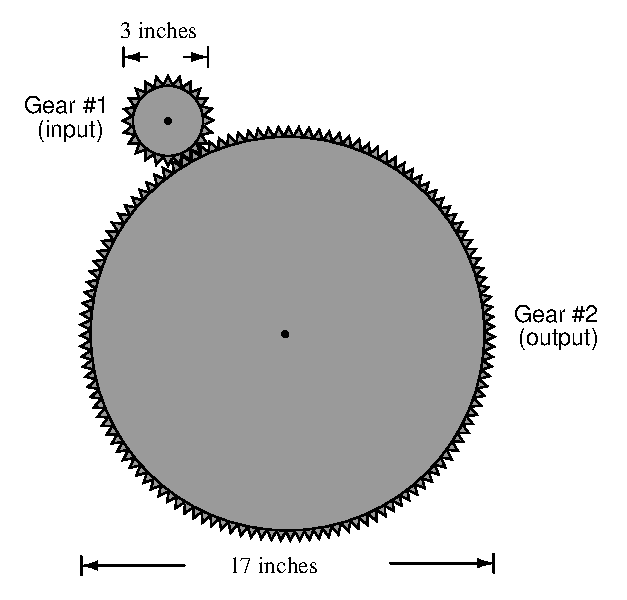
\includegraphics[width=15.5cm]{i01405x01.eps}$$

Basert på dette diagrammet av de to tannhjulene, svar på disse spørsmålene:

\begin{itemize}
\item{} Beregn {\it utvekslingen} for dette tannhjulsparet.
\vskip 10pt
\item{} Hvis akselen til det første tannhjulet påfører tannhjulet et dreiemoment på 600 lb-ft (``inngangs''-moment), hvor stort dreiemoment vil da påføres akselen til det andre tannhjulet (``utgangs''-moment)?
\vskip 10pt
\item{} Hvis inngangshjulet roterer med 200 RPM, hvor fort roterer utgangshjulet?
\vskip 10pt
\item{} Hvis det lille tannhjulet har 24 tenner, hvor mange tenner vil det store tannhjulet ha?
\end{itemize}

\vskip 20pt \vbox{\hrule \hbox{\strut \vrule{} {\bf Forslag til sokratisk diskusjon} \vrule} \hrule}

\begin{itemize}
\item{} Bruk momentformelen $\vec \tau = \vec r \times \vec F$ (dreiemoment som produkt av radius og lineær kraft) til å løse for momentforholdet $\left( \tau_1 \over \tau_2 \right)$ når du kjenner diameterforholdet (eller radiusforholdet) mellom to inngrepende tannhjul.
\item{} Bruk hastighetsformelen $v = r\omega$ (randhastighet som produkt av radius og rotasjonshastighet) til å løse for rotasjonshastighetsforholdet $\left( \omega_1 \over \omega_2 \right)$ når du kjenner diameterforholdet (eller radiusforholdet) mellom to inngrepende tannhjul.
\end{itemize}

\underbar{file i01405}
%(END_QUESTION)





%(BEGIN_ANSWER)

\noindent
{\bf Delvis svar:}

\begin{itemize}
\item{} Hvis akselen til det første tannhjulet påfører tannhjulet et dreiemoment på 600 lb-ft (``inngangs''-moment), hvor stort dreiemoment vil da påføres akselen til det andre tannhjulet (``utgangs''-moment)?  {\it $\tau_{output}$ = 3,400 lb-ft}
\vskip 10pt
\item{} Hvis det lille tannhjulet har 24 tenner, hvor mange tenner vil det store tannhjulet ha?  {\it 136 tenner}
\end{itemize}
 
%(END_ANSWER)





%(BEGIN_NOTES)

\begin{itemize}
\item{} Beregn {\it utvekslingen} for dette tannhjulsparet.  {\it Utveksling = 17/3 = 5.667:1}
\vskip 10pt
\item{} Hvis akselen til det første tannhjulet påfører tannhjulet et dreiemoment på 600 lb-ft (``inngangs''-moment), hvor stort dreiemoment vil da påføres akselen til det andre tannhjulet (``utgangs''-moment)?  {\it $\tau_{output}$ = (600 lb-ft)(17/3) = 3,400 lb-ft}
\vskip 10pt
\item{} Hvis inngangshjulet roterer med 200 RPM, hvor fort roterer utgangshjulet?  {\it $S_{output}$ = (200 RPM)(3/17) = 35.29 RPM}
\vskip 10pt
\item{} Hvis det lille tannhjulet har 24 tenner, hvor mange tenner vil det store tannhjulet ha?  {\it (24)(17/3) = 136 tenner}
\end{itemize}

%INDEX% Physics, torque: definition
%INDEX% Physics, torque: calculation problem

%(END_NOTES)

